%Master document for paper.
%Created MS 4/12

\documentclass[12pt,notitlepage]{article}

\usepackage[text={6.5in,9in},centering]{geometry}               % See geometry.pdf to learn the layout options. There are lots.
\geometry{letterpaper}                   % ... or a4paper or a5paper or ... 
%\geometry{landscape}                % Activate for for rotated page geometry
\usepackage[parfill]{parskip}    % Activate to begin paragraphs with an empty line rather than an indent
\usepackage{subfigure}
\usepackage{graphicx}
\usepackage{setspace}
\usepackage{color}
\usepackage{amssymb}
\usepackage{amsmath}
\usepackage{listings}
\usepackage{epstopdf}
\usepackage{epsfig}
%\usepackage{psfig}
\usepackage[dvips, bookmarks, colorlinks=true, linkcolor=blue, citecolor=blue, pdftitle={Investigation of the Properties of Superfluid He4}, pdfauthor={Baryakhtar, Schowalter, Swiatlowski}, pdfsubject={Physics 191 Lab Report}, pdfkeywords={helium, superfluid, physics, 191}]{hyperref}
\DeclareGraphicsRule{.tif}{png}{.png}{`convert #1 `dirname #1`/`basename #1 .tif`.png}
\usepackage{cite}

\begin{document}

%\title{Investigation of the Properties of Superfluid He$^4$}
%\author{Maria Baryakhtar \footnote{Produced Introduction and
%    Background (Sections \ref{introduction}, \ref{background}),
%    Appendix ~\ref{masscalibration}, and Abstract} \and Steven
%  Schowalter \footnote{Produced Results and Discussion (Section
%    \ref{resultsanddiscussion}) and Appendix
%    ~\ref{muontimeerroranalysis}} \and Maximilian Swiatlowski
%  \footnote{Produced Instrumentation and Procedure (Sections
%    \ref{instrumentation}, \ref{procedure})}}

%\maketitle
%\thispagestyle{empty}

\begin{titlepage}
\begin{center}
\ \\
\vspace{1in}

{\Huge
Investigation of the \\ Properties of Superfluid $^{4}$He
\\}
\ \\

%\large{In partial fulfillment of the requirements of Physics 191r at Harvard University}

Maria Baryakhtar \footnote{Harvard University, Cambridge MA 02138 \\ \qquad \qquad Masha Baryakhtar produced the Background~(\ref{background}) and Conclusion~(\ref{conclusion}) sections, and the superfluid fraction calculation~(\ref{superfluiddensity}). \\ \qquad Steven Schowalter produced the Results~(\ref{results}) and Analysis~(\ref{analysis}) sections and the Appendices. \\ \qquad Maximilian Swiatlowski produced the Abstract, Introduction~(\ref{introduction}), and Experimental~(\ref{experimental}) sections.}, Steven Schowalter \footnotemark[\value{footnote}], Maximilian Swiatlowski \footnotemark[\value{footnote}] 

\ \\

%Abstract body
%Created MB 04-12

%\section{Abstract}\label{abstract}

%formatting inserted by MS so that it works with the new title page. (Yes, I know that the center thing looks funny, but it works ;) )
%\begin{bfseries}
%Abstract
%\end{bfseries}

\end{center}

\begin{abstract}
%put text of the abstract here
  We present our measurements and observations of several different
  properties of superfluid $^{4}$He. Liquid helium is lowered to
  superfluid temperatures, below the $\lambda$-point $T_{\lambda}$, by
  lowering the vapor pressure with a pumping system. Observations of
  the transition to the helium II state and the `fountain effect' are
  conducted through a glass viewport. The velocity of second sound,
  \emph{i.e.} temperature waves, is measured as a function of
  temperature by recording the travel time of heat pulses. The
  specific heat of helium around $T_{\lambda}$ is found by measuring
  the temperature response to a fixed heat pulse. Both measurements
  are in very good agreement with established measurements
  \cite{atikins}. The $\lambda$-point itself is calculated to be
  $T_{\lambda} = 2.178\pm0.081$ K, in excellent agreement with the
  established value \cite{atkins}. Finally, using the second sound
  velocity and specific heat values, the fractions of superfluid and
  normal fluid helium are calculated as a function of temperature, in
  strong agreement with prior experiments\cite{andro}.
\end{abstract}

\begin{center}


\end{center}
\end{titlepage}

\clearpage

%Introduction body
%Created MS 1-30

\section{Introduction}\label{introduction}

The muon, a fundamental particle produced in the upper atmosphere as a
secondary product of cosmic ray collisions, was originally discovered
in 1936 \cite{}. It decays via the weak interaction with a mean decay
lifetime of $2.2 \mu s$, longer than every known particle other than
the neutron \cite{}. With muons comprising $80$\% of cosmic ray flux at
sea level, the muon is a good candidate for the study of the weak
force \cite{}.

Our experiment consists of two main components: the muon lifetime
measurement and the muon mass measurement. In section 2,
\emph{Background}, we introduce the theoretical basis for these
measurement as well as that of muon creation and decay. We describe
the experimental setup which consists of a system of three
scintillators and photomultiplier tubes (PMTs) in \emph{Setup}. Using
this system, the cosmic ray muons passing through the scintillators
and their decay products can be detected along with their enegy
(\emph{Procedure}). The muon lifetime and mass results are presented in
\emph{Results} and \emph{Discussion} with the relevant statistical
analysis of data, and compared to previous experimentally established
values. Finally, we use the muon mass and lifetime values to calculate
the weak force coupling constant, $g_w$.


%Background body
%Created MB 04-12

\section{Background}\label{background}

The $^4$He atom is one of the very simple and symmetrical systems
among the elements, with a filled innermost electron shell and no
overall electric or magnetic moment or angular momentum to the atom
\cite{atkins}. Due to the symmetric nature of helium atoms, the
interaction between them is very weak, and $^4$He liquifies at an
extremely low temperature of $4.21$ K. However, a more interesting
transition occurs at $2.17$ K, at which point liquid helium takes on
several unique properties. Below this temperature, termed the
$\lambda$ point, $^4$He\footnote{Although the isotope $^3$He is also
  capable of producing these effects, the transition temperature is
  much lower at $3\times 10^{-3}$ K and is unreachable with the
  cryogenic technology available to us. Thus, in the remainder of the
  paper, the isotope $^4$He is implied unless stated otherwise.}
acquires extremely high thermal conductivity, negligible viscocity,
and the ability to propagate temperature waves(second sound); in
addition, there is a $\lambda$-shaped discontinuity at the transition
in the heat capacity of liquid helium, which is how the $\lambda$
point acquires its name. To distinguish the two phases of liquid
helium, the liquid is referred to as helium I above the lambda point
and helium II below the lambda point (BLAHHH). The investigation of
the properties of helium II mentioned above will be the focus of this
paper.

\subsection{The Two-Fluid Model}

A key model explaining the unusual properties of He II was proposed by
Landau in 1941 as the two-fluid model \cite{landau}. In this theory,
the liquid below the $\lambda$-point can be viewed as being composed
of two noninteracting fluids: a superfluid component with density
$\rho_s$ and a normal component with density $\rho_n$, such that the
total density $\rho$ is given as the sum of the two components:
\begin{equation}
\rho = \rho_s + \rho_n
\end{equation}

and the total current density of He II is given by
\begin{equation}
\mathbf{j} = \rho_s\mathbf{v_s} + \rho_n\mathbf{v_n}
\end{equation}

where $\mathbf{v_s}$ and $\mathbf{v_n}$ are the velocities of the
superfluid and normal fluid, respectively \cite{tilley}. Then, the
behavior of the fluid can be understood in terms of the different
characteristic of the two components: while the normal fluid acts
according to the regular laws of fluid mechanics and satisfies the
Navier-Stokes equation, the superfluid has zero entropy and flows with
zero viscocity. Furthermore, it is important to note that the two
components are non-interacting, that is, there is no transfer of
momentum between the two fluids, and most importantly that they are
not physically distinct and cannot be separated \cite{tilley}.

With the incorporation of theories of Bose-Einstein condensates into
Landau's theory, further understanding of the fluid is possible. The
superfluid can be viewed as an interacting Bose-Einstein condensate
system, occupying a single macroscopic quantum state, whereas the
normal fluid consists the excitations (photons and rotons) of the
superfluid. As temperature decreases from $2.17$ to $0$ K, the
fraction of superfluid increases, from $0$ at the $\lambda$-point to
unity at absolute zero, as the excitations decrease to zero.

\begin{figure}[ht]
\begin{center}
%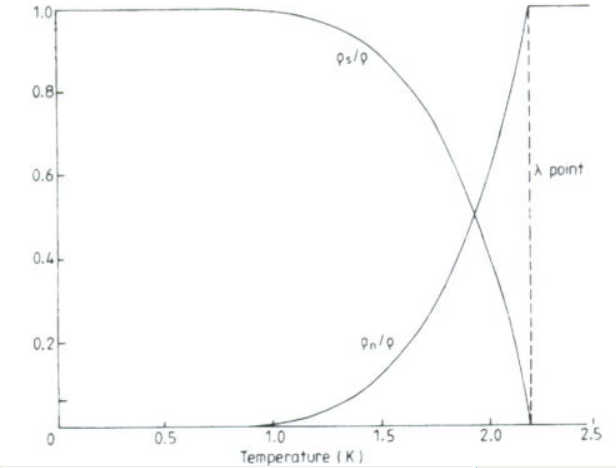
\includegraphics{./figures/twofluid.eps} WHY NOT WORKINGGGGGGG
%\{./figures/twofluid.eps}
\caption{\small{Relative fractions $\rho_s/\rho$ and $\rho_n/\rho$ of
    the superfluid and normal components in He II.}}
\label{figure:twofluid}
\end{center}
\end{figure}



\subsection{Second Sound}

The thermal conductivity of He II is very high, and tends to infinity
for small heat currents \cite{tilley}. This makes the fluid intolerant
to temperature gradients. This property explains the visually
noticeable transition from He I to He II with descreasing temperature:
while in He I, there is a lot of bubbling, as the temperature passes
the $\lambda$-point, the bubbling ceases immediately, since a
temperature gradient large enough cannot be established in order for a
bubble to form \cite{tilley}.

Interestingly, the superfluid fraction cannot transfer heat, but is
able to balance temperature gradients not through convection and
BLAHHOTHERTHING but through an exchange of the relative concentrations
of the two componenets $\rho_n$ and $\rho_s$. As seen in FIGURE
TWOFLUID, at lower temperatures the fraction of superfluid increases.

The relationship between velocity of second sound, $u_2$, and the
relative fractions of the fluids was derived analytically by Landau
and is given by

\begin{equation}
u_2^2 = \frac{\rho_s}{\rho_n}\frac{T S^2}{C}
\end{equation}

where $S$ and $C$ are the entropy and heat capacity per gram of the
liquid and can be measured experimentally \cite{atkins}. 

\subsection{Heat Capacity}


%Experimental body
%Created MB 04-12

\section{Experimental}\label{experimental}

The experiment constists of three main components: direct observation
of the visual properties of liquid helium, measurement of second sound
velocity as a function of temperature, and measurement of specific
heat as a function of temperature. Several features are common to all
three experiments performed. Two separate Precision Cryogenic Systems
model PVS-337 LHe Vapo-Shield Dewars are used for different stages fo
the experiment. Aluminized Mylar superinsulation provides isolation to
the external environment. The preparatory procedure for all
experiments is to precool the dewar to $77$ K using liquid nitrogen
and then to fill the dewar with liquid helium. Temperature control of
the liquid helium is achieved by pumping on the liquid with a
mechanical vacuum pump: changing the vapor pressure also changes the
temperature in a predictable manner, subject to a calibration found in
\ref{temperaturecalibration}. The temperature of helium I is uniform
throughout the bath if the system is being pumped down (that is, for
decreasing temperature); the temperature of helium II is uniform
constantly, as described in Section~\ref{thermalconductivity}.

\subsection{Visual Observation Experiments}

The first experiment consists of visual observations of superfluid
helium phenomena. One helium dewar has a glass observation window near
the bottom; while this increases coupling to the environment and
thereby raises the lowest achievable temperature, it is still possible
to pump the helium down to superfluid temperatures and enables direct
observation of the liquid.

\subsubsection{Transition between He I and He II}

The most obvious phenomenon is the transition between helium I and helium II. As the temperature is lowered through the $\lambda$-point, it is possible to observe through the window the marked change in the appearance of the liquid, which is a result of helium II's inability to support temperature gradients as described in Section \ref{thermalconductivity}.

\subsubsection{Superfluid fountain}\label{superfluidfountain}

The next experiment allows for a particularly impressive display of this inability to support temperature gradients. A specially crafted glass container has a very narrow capillary tube on top, and a wide semi-porous glass bottom. The semi-porous glass (made of very finely ground and compacted glass) creates winding openings of diameter on the order of $100$ $\mu$m which allow only superfluid, not normal fluid, to pass. A $100$ $\Omega$ resistor placed inside the container acts as a heater. When a potential difference is applied to the resistor, the heated helium draws cooler superfluid to it in an effort to remove the temperature gradient; this sudden rush of superfluid forces some fluid out through the capillary tube on top, creating a small helium fountain.

\subsection{Second Sound Experiment}

In the second part of the experiment, we measure the propagation speed of second sound as a function of temperature.

A grid of Nichrome wire, with a resistance of about $10$ $\Omega$, is
used as a resistive heater to produce heat pulses. A HP3018A function
generator creates an $80$ $\mu$s low voltage ($5$ V) pulse, which is
amplified to $40$ V with a Kepco BOP 50-2M Power Amplifier and sent to
the heater.

To measure second sound propagation speed, a thermometer is necessary
to detect the signal produced by the heater. A carbon resistor ($65$
$\Omega$ at room temperature) is supplied with a constant $100$ $\mu$A
current, and the potential difference across it is read by a
voltmeter. A change in temperature of the resistor at very low
temperatures corresponds to a change in resistance, and therefore a
change in potential difference. This resistor (referred to as a
bolometer) is placed at the end of a sliding rod, whose distance from
the Nichrome wire is able to be adjusted from $3$ cm to $12$ cm.

A heat pulse read on the bolometer is expected to be visible as a dip
on an oscilloscope. As temperature increases when the heat pulse
passes the bolometer, the resistance decreases, and therefore the
potential difference decreases. The signal from the bolometer is very
noisy and difficult to read, as the wires leading to it are unshielded
so as to lower thermal contact into the liquid helium. A $60$ Hz
bandpass filter reduces powerline pickup, the worst source of noise;
to remove other sources of noise and to amplify the signal, a EG\&G
PARC 113 Pre-Amp is set to a gain of $10^4$ with a $3\times 10^3$ Hz
high-pass filter and $0.1$ Hz low-pass filter.

To perform each measurement at a constant temperature, it is important to maintain the vapor pressure at a constant level. A series of valves attached to the vacuum pump allows for very fine control of the pumping rate, which can be set at a level to temporarily balance the heat flow from the outside environment. Changes in volume of the liquid offset this delicate equilibrium, so it is necessary to constantly monitor the pressure and update the pumping rate to compensate.

In order to calculate the second sound velocity, first a constant temperature is selected. A series of heat pulses are sent using the function generator, and an oscilloscope is set to average over $128$ measurements of the response from the bolometer to further increase signal to noise. The distance between the wire and the bolometer is recorded as well as the time between the pulse from the generator and the first dip on the bolometer; this time corresponds to how long it took the pulse to travel from the nichrome wire to the bolometer. The bolometer distance is then altered, and the measurement repeated. Once $7$ measurements are taken at one temperature, the temperature is changed and the process is repeated.

\subsection{Heat Capacity Experiment}\label{heatcapacityexperiment}

The purpose of the next experiment is to determine the specific heat
of liquid helium as a function of temperature; to measure this
dependence, a predetermined heat pulse is sent into a high purity sample
of liquid helium contained in a small copper cell and the temperature
response is measured at different initial temperatures.

\subsubsection{Thermometer Calibration}\label{thermometercalibration}

As in the second sound experiment, a resistor attached to the cell is
used to monitor changes in temperature. Unlike the second sound
experiment, the resistor used is composed of germanium, which has
predictable behavior as a function of temperature and excellent
cycling properties (that is, one measurement of a resistance will
always correspond to the same temperature, as there is little drift
between experimental runs). A constant current of $1.00$ $\mu$A is
applied to the thermometry resistor by tuning the voltage of the power
supply and reading the electric potential drop across a fixed $9.963$
k$\Omega$ resistor at room temperature which is in series with the
thermometer. The potential difference across the thermometry resistor
is then amplified by an operational amplifier circuit with a gain of
170 so as to increase the signal and decrease output impedance.\footnote{Note that the maximum current is limited by the maximum
  output voltage of the op-amp, 4.4 V. While it would be ideal to
  use a higher current in order to increase resolution of the
  potential difference measurement, since the error is $\delta V
  \propto \frac{V}{I} \delta I$ and therefore goes down with increased
  current, the op-amp enforces a maximum of 1 $\mu$A to avoid
  saturation.}

A large volume of exchange gas is introduced into the the inner vacuum
can in order to couple the temperature of the cell (and thereby the
cold resistor) with the temperature of the helium bath. Such a large
amount is necessary because of the activated charcoal cryopumps
placed in the vacuum can: these must be saturated to provide proper
coupling. As the temperature decreases, the efficiency of the cryopump
increases, so it is important to monitor the pressure of this exchange
gas and ensure that it is always present. The potential difference
across the germanium resistor and the vapor pressure of the helium
bath are recorded as the helium is pumped down to equilibrium. Pumping
is paused as each potential difference measurement is taken, allowing
the systems to thermally equilibrate. After adjusting values of the
recorded pressure for known offsets in the gauges, the potential
difference is fit against temperature with the function

\begin{equation}
\label{eq:fiteqn}
\ln{V} = \sum_{n=0}^{8} a_{n} (\ln{T})^{n}
\end{equation}

recommended by White for fitting the resistance of germanium as a
function of temperature \cite{white}. Note that we fit potential,
which is only different from resistance by the constant factor of $I$,
changing the constants but not the overall form of
Eqn.\ref{eq:fiteqn}.

\subsubsection{Heat Pulses}

Once the germanium resistor successfully calibrated, the next step is
to send constant heat pulses into the system. A second resistor is
placed onto the copper cell to function as a heating element. A four
probe measurement of the resistance is taken; for a potential
difference pulse of a set duration and amplitude, the output heat is given by

\begin{equation}
Q = P \Delta t = V^{2} \Delta t /R
\end{equation}
where $V$ is the magnitude of the pulse, $\Delta t$ is the duration,
and $R$ is the resistance. Note that the electric potential here is
read off from the 4-probe measurement as well, not from the voltage
source itself, in order to cancel the resistance of the long wires
down to the resistor. An electronics system sends out pulses with
adjustable amplitude and duration, so the rate of pulses and amount of
heat per pulse can be precisely regulated.


\subsubsection{Heat Capacity of Copper Cell}

Before the specific heat of helium can be determined, it is necessary
to measure the heat capacity of the empty copper cell. To begin, we
pump down the system to the lowest temperature possible. At this point
the inner vacuum is still empty, so the cell is still at room
temperature. A moderate amount of helium buffer gas is introduced into
the vacuum can, which the cryopump quickly absorbs. A heater attached
to the cryopump is then activated (and the temperature monitored on a
diode thermometer) so as to desorb the cryopump and allow the copper
cell to equilibrate with the helium bath at the very low
temperature. The heater is then turned off and the buffer gas absorbed
by the cryopump, so the copper cell is isolated from the bath. Because
the capillary leading out is very small, coupling to the outside
environment is minimal, though not completely negligible. The potential
difference across the germanium resistor is recorded by a computer,
and pulses of heat are sent into the cell. Sufficient time is allowed
between pulses for the system to equilibriate. With a given heat pulse
and a measured temperature response per pulse, the heat capacity of
the copper cell (as a function of temperature) can be calculated and
fit to a theoretical curve, as described in \ref{specificheatofmetals}.

\subsubsection{Specific Heat of Helium}
In order to measure the specific heat per mole of helium, the number
of moles in the high purity sample must be established. The helium is
stored in a container of known volume at room temperature; once the
pressure is measured, the ideal gas law $P V = n R T$ gives the number
of moles $n$. Next, the system is cooled to the lowest achievable
temperature and the cell is brought into thermal contact with the bath
using the procedure described above. The helium from the container is
then allowed into the capillary connecting it to the cell; because
liquid helium is $760$ times as dense as gaseous helium at a given
pressure \cite{shi}, almost all of the helium condenses into the cell,
and the only gas that remains is from vapor pressure of the liquid at
this low temperature. 

The cryopump heater is then turned off so as to isolate the system,
and predetermined heat pulses are sent into the cell through the
heater.\footnote{We make the approximation that all the helium
  becomes liquid, and that this is true for all the relevant
  temperatures. This assumption introduces a minor error, as the vapor
  pressure does change and the amount of gaseous helium therefore also
  changes, but this is a negligible effect compared to the factor of
  $760$ discussed previously.} The potential difference across the
thermometer is once again read and recorded by a computer. It is
particularly important at this step to ensure that enough time has
been provided for the system to equilibrate after each pulse; while
helium II does not support temperature gradients and therefore
equilibrates quickly because the copper is the relevant time constant,
helium I takes much longer to reach steady temperature. Given that
there is an element of heating through the capillary which couples the
system to room temperature, it is also important ensure the time
between pulses is short enough such that the heating does not affect
measurements.  Once the heat capacity of the entire system is
calculated, the heat capacity of the copper is subtracted and the
result divided by the number of moles, so as to obtain the molar
specific heat of the helium alone.


%Conclusion body
%Created SS 04-14

\section{Results}
\label{results}

\subsection{Observation}
\subsubsection{$\lambda$-point Transition}
As the temperature of liquid helium was decreased, we witnessed rapid
bubbling of the fluid. The bubbling ceased immediately as the
temperature passed $T_{\lambda}$, confirming the intolerance of helium
II to thermal gradients.

\subsubsection{Fountain Effect}
We observed a small stream of liquid helium emerging from the
capillary of the `fountain' system, described in Section
\ref{superfluidfountain}. The fountain is only visible at temperatures
below the $\lambda$-point, and the height of the stream decreases with
increasing temperature. This provides a good visual demonstration of
the decreasing fraction of superfluid as temperature of the system
approaches $T_{\lambda}$ from below.

\subsection{Second Sound Results}
\label{secondsoundresults}

To measure the velocity of second sound in He II, the propagation time of heat pulses in the superfluid is observed over a range of temperatures. First the displacement between the bolometer and the heater (both fully submerged) is measured. Next, heat pulses sent from the heater propagate towards the bolometer as second sound. The duration between the triggering of the heat pulse and the pulse's signature recorded by the bolometer was observed and recorded. Multiple displacements and corresponding durations were recorded for various temperatures ranging from $1.6$ K to $2.2$ K, shown in Figure \ref{fig:secondsoundraw}. Second sound velocity goes to zero as the temperature approaches $T_{\lambda}$.


\begin{figure}[htbp]
\begin{center}
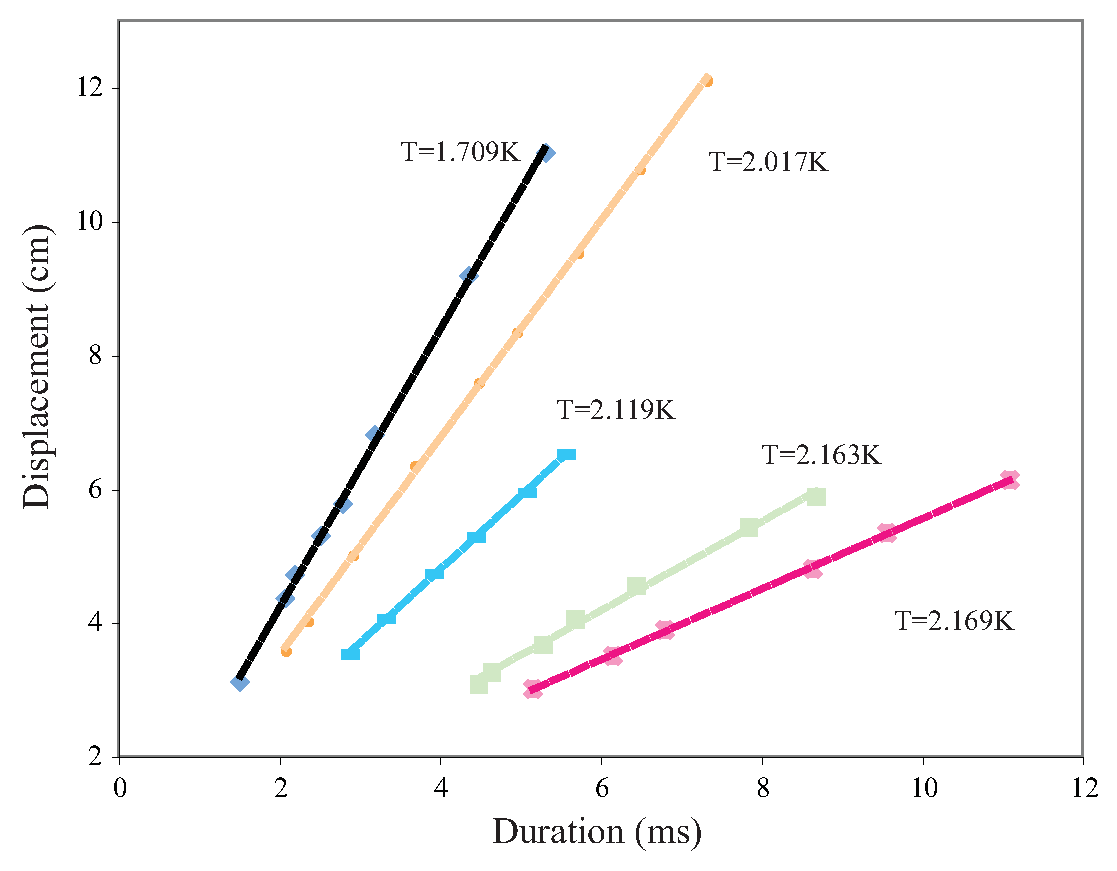
\includegraphics[height=70mm]{./figures/secondsoundraw.eps}
\caption{\small{A plot of the displacement of the thermometer from the heater \emph{versus} the duration between the triggering of the heat pulse and the pulse's signature recorded by the thermometer for various temperatures in He II.}}
\label{fig:secondsoundraw}
\end{center}
\end{figure}


\subsection{Heat Capacity Results}\label{heatcapacityresults}

To measure heat capacity, we observe the effect of heat pulses sent to the cell on a germanium resistor which is thermally coupled to the cell. Beginning at a temperature of about $1.8$ K, $10$ ms heat pulses with a power of $98.8$ mW were sent to the cell.  These heat pulses caused the temperature of the cell to rise which consequently caused the resistance of the coupled germanium resistor to increase.  Because the current through the germanium resistor is a constant $1.00$ $\mu$A, a decrease in resistance causes a decrease in the potential difference across the resistor. The change in the potential difference due to consecutive heat pulses sent to the cell was measured while the copper cell was both filled and evacuated. Figure \ref{fig:rawdata} shows portions of this data for both scenarios.  Over the course of the experimental run, the potential difference in both cases falls in discrete sections due to the consecutive heat pulses. While the changes in potential per heat pulse are uniform in the empty cell for the entire observed temperature range, the changes in potential difference for the filled cell depend upon whether the temperature of the cell is above or below $T_{\lambda}$. This disparity is shown in Figure \ref{fig:rawdata}. 

\begin{figure}[htbp]
\begin{center}
\subfigure[Cu Addendum]{\label{fig:edge-a}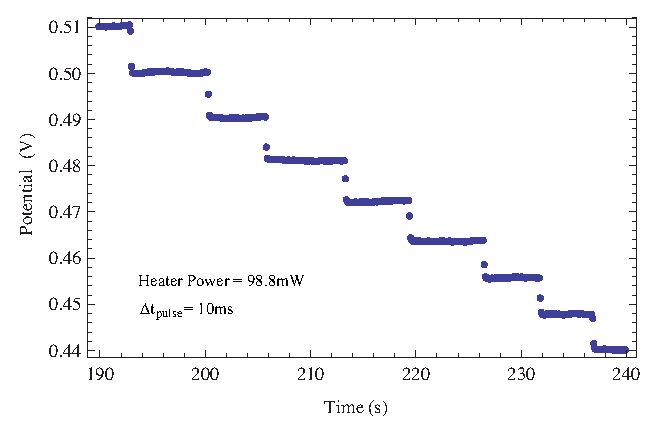
\includegraphics[height=52mm]{figures/rawcu.eps}}
\hspace{-1mm}
\vspace{-2mm}
\subfigure[He II and Cu Addendum near $T_{\lambda}$]{\label{fig:edge-b}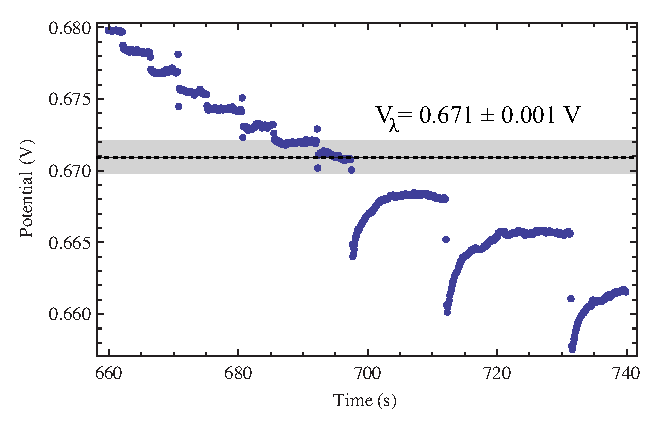
\includegraphics[height=52mm]{figures/rawhe.eps}}
\vspace{-2mm}
\caption{\small{Plots showing the change in the thermometer's potential difference due to heat pulses sent to (a) the evacuated addendum and (b) the addendum filled with HeII.  Each heat pulse is $10$ ms with a power of $98.8$ mW.  From this data we see that $T_{\lambda}$ occurs at $0.671 \pm 0.001$ V judging by the sudden change of the heat pulse's signature.}}
\label{fig:rawdata}
\end{center}
\end{figure}

Knowing the amount of energy deposited in the cell along with the change in temperature, we can calculate heat capacity of the evacuated copper cell and the copper cell filled with helium. To calculate the heat capacity of only the helium, we subtract the heat capacity of the evacuated cell from the heat capacity of the filled cell.

%analysis body
%Created MB 04-12

\section{Analysis}\label{analysis}
\subsection{Second Sound Analysis}\label{secondsoundanalysis}

By analyzing the second sound data shown in Figure \ref{fig:secondsoundraw}, we can determine the relationship between the temperature of He II and the propagation speed of second sound.  By using linear regression analysis, we can determine the slope of each temperature data set.  For each of the fifteen data sets, the $r^{2}$-value is greater than $0.99$.  The values for the slope of these fits, in m/s, correspond to the propagation speed of second sound in the respective temperature.  These speeds can then be plotted against temperature in order to show the relationship between the two in He II.  Figure \ref{fig:secondsound} shows the relationship between second sound speed and temperature in He II.  This data is compared to results made by Peshkov.\cite{peshkov}

\begin{figure}[htbp]
\begin{center}
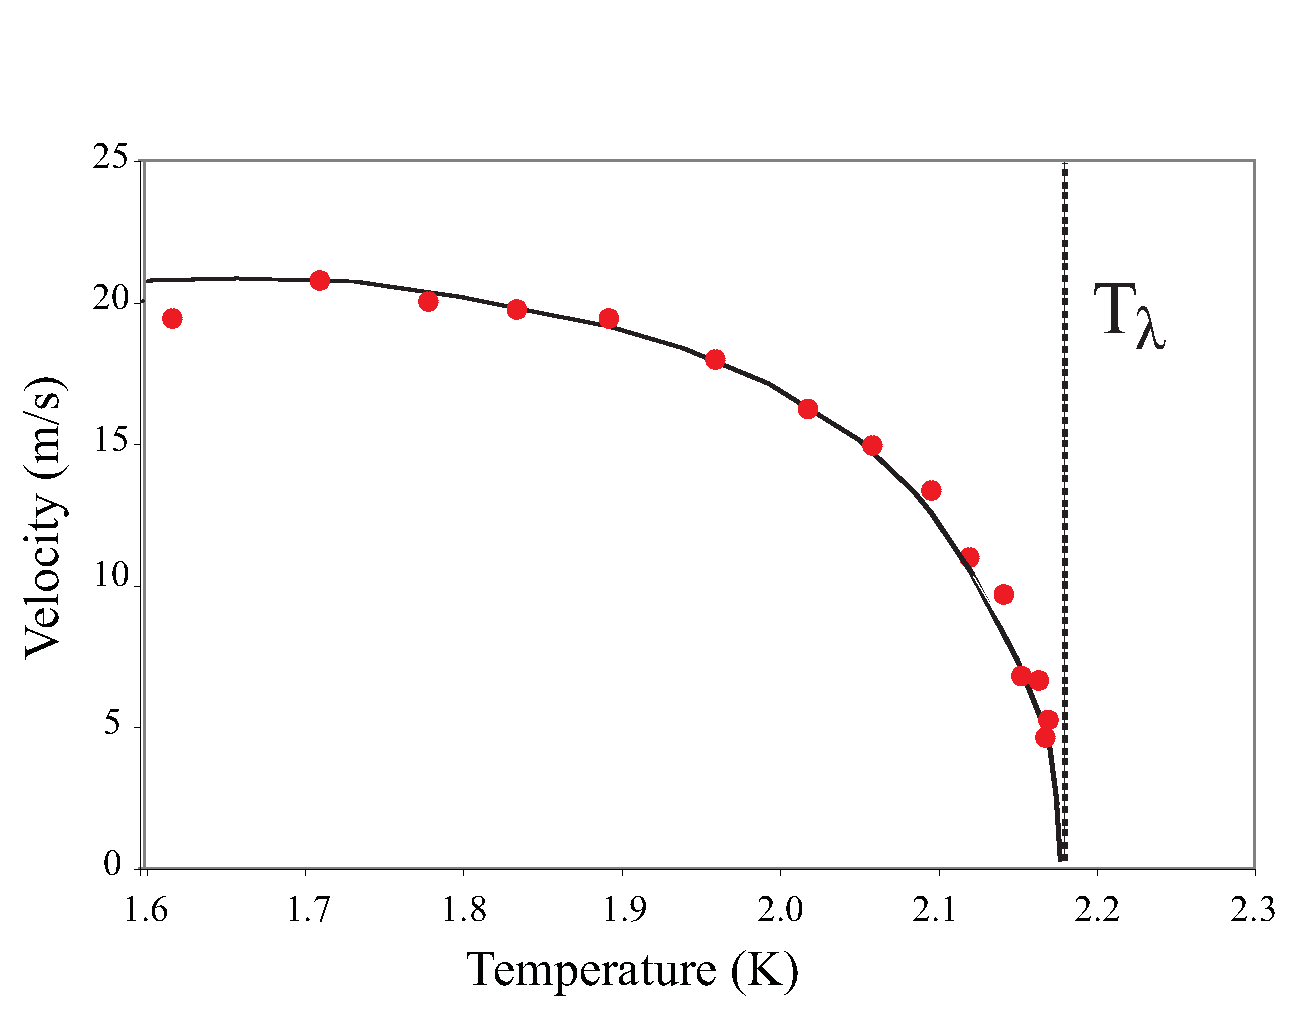
\includegraphics[height=70mm]{./figures/secondsound.eps}
\caption{\small{A plot of the second sound speed verses temperature in He II.  This data is compared to Peshkov's results.\cite{peshkov} Second sound velocity goes to zero at the transition from He II to He I enabling a rough estimate of $T_{\lambda}$.}}
\label{fig:secondsound}
\end{center}
\end{figure}

The statistical error of the speeds is due to statistical measurement error, resulting in a relative error of $2.1\%$. To eliminate systematic error in second sound calculations, we calculate the slope of several measurements of time delay \emph{vs.} measured displacement of the bolometer. This method avoids systematic offsets to either the time delay or the displacement and instead emphasizes the relative differences between data points. As a result, the error in second sound speed is purely statistical (see Appendix \ref{errorinsecondsoundcalculation} for further error analysis).

\subsection{Heat Capacity Analysis}\label{heatcapacityanalysis}
\subsubsection{Temperature Calibration}\label{temperaturecalibration}

In order to measure heat capacity, we must be able to measure the temperature of the cell.  Because the germanium resistor is thermally coupled to the cell, we can use it as a thermometer for the cell.  Thus the potential difference across the resistor must be converted to temperature.  Following the procedure described in Section \ref{thermometercalibration}, data relating the potential difference across the resistor to the temperature of the cell is produced.  This data can then be fit to a curve given by Equation \ref{eq:fiteqn} in order to determine an expression for temperature as a function of electric potential.  This data with the fit is shown in Figure \ref{fig:polyfit}.  

\begin{figure}[htbp]
\begin{center}
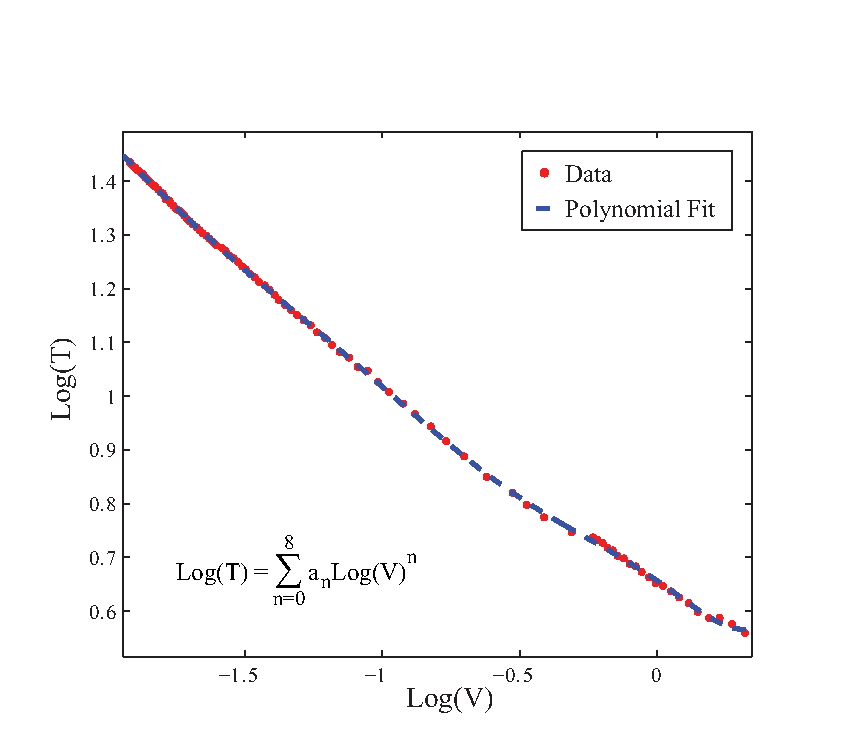
\includegraphics[height=70mm]{./figures/polyfit.eps}
\caption{\small{This plot show the log-log relationship between the potential difference across the germanium resistor and the temperature of the cell for temperatures ranging between $1.8$ K and $4$ K.  The fit is based on Equation \ref{eq:fiteqn} resulting in an $8^{th}$-degree polynomial using nonlinear regression analysis.  The resultant $r^{2}$-value is $0.999$.}}
\label{fig:polyfit}
\end{center}
\end{figure}

The fit was computed doing a $8^{th}$-degree polynomial regression (see Appendix \ref{nonlinearregressionanalysis}) of the log-log data and found to be 
\begin{eqnarray}\label{eq:polyfit}
\ln(T) &=& 0.6568 - 0.3503\ln(V) - 0.1635\ln(V)^{2} + 0.2846\ln(V)^{3} \\
& & + 1.813\ln(V)^{4} + 2.521\ln(V)^{5} + 1.593\ln(V)^{6} + 0.4845\ln(V)^{7} + 0.0578\ln(V)^{8} \nonumber
\end{eqnarray}

where $T$ is the temperature of the cell and $V$ is the potential difference across the germanium resistor.  Relative uncertainties in the fitting parameters of this polynomial add to the relative error in calculated temperatures.   

\subsubsection{Calculating the Heat Capacity of Helium}\label{calculatingtheheatcapacityofthecell}

In order to calculate heat capacity from the data shown in Figure \ref{fig:rawdata}, the potential difference across the germanium resistor must be converted to temperature using Equation \ref{eq:polyfit} determined in Section \ref{temperaturecalibration}. A portion of the sample data after being converted from potential to temperature is shown in Figure \ref{fig:heatingdata}.  

\begin{figure}[htbp]
\begin{center}
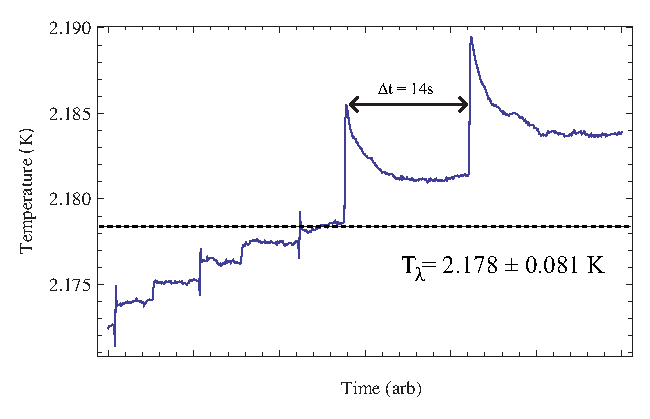
\includegraphics[height=70mm]{./figures/heatingdata.eps}
\caption{\small{A plot of the data from Figure~\ref{fig:rawdata} (b) after being converted from electric potential to temperature using the calibration in Section \ref{temperaturecalibration}.  From this data, $T_{\lambda}$ is determined to be $2.178\pm0.081$ K.}}
\label{fig:heatingdata}
\end{center}
\end{figure}

By analyzing data shown in Figure \ref{fig:rawdata} (b) and using Equation \ref{eq:polyfit}, we can determine the value for $T_{\lambda}$ from $V_{\lambda}$, which is defined as the potential difference across the germanium resistor at which which the He within the cell transitions form a superfluid to a fluid. 

As the temperature of He II heats to $T_{\lambda}$, the change in temperature, $\Delta T$, decreases for a constant heat pulse $Q$.  This implies that the change in electric potential, $\Delta V$, decreases as it heats to $V_{\lambda}$.  The transition from He I to He II is denoted by a change in the heat pulse's signature.  As seen in Figure \ref{fig:rawdata}, $\Delta V$ transitions from discrete steps to discrete exponentially decaying steps.  This signature is repeated after converting electric potential to temperature as shown in Figure \ref{fig:heatingdata}.  The reason for this change in signature is due to the drastic divergence of the heat capacity of helium at $T_{\lambda}$.  For temperatures less than $T_{\lambda}$, the energy of the heat pulse sent to the cell is immediately absorbed uniformly in the He II due to the inability of superfluids to have temperature gradients.  This corresponds to the discrete steps we see in Figures \ref{fig:rawdata} and \ref{fig:heatingdata}.  For temperatures greater than $T_{\lambda}$, the liquid helium, no longer in its superfluid state, can support temperature gradients.  As a result, the heat pulse is not immediately absorbed by the helium and the time constant describing the transfer of heat from the copper cell to the contained helium is much longer. This results in an exponential cooling curve as we see in Figures \ref{fig:rawdata} and \ref{fig:heatingdata}.  

From this analysis, we can determine the range in which $T_{\lambda}$ occurs: \emph{i.e.}, between the temperatures which we know correspond to either He I or He II.  More precisely, we know that a heat pulse followed by discrete step in electric potential (or temperature) is the signature of He II, while an exponentially decaying signature corresponds to He I. Therefore the transition must lie in between these signatures.  Observing our measured electric potential data in Figure \ref{fig:rawdata}, the interval for $V_{\lambda}$ must be as shown.  With Equation \ref{eq:polyfit}, we can convert this potential to temperature in order to determine $T_{\lambda}$.  Figure \ref{fig:heatingdata} shows the interval for $T_{\lambda}$, which we calculate as $2.178\pm0.081$ (see Appendix \ref{errorinspecificheatcalculation} for error analysis). 

To calculate heat capacity we use the converted temperature data in order to determine the cell's change in temperature, $\Delta T$, caused by a heat pulse with known energy $Q$, from some initial temperature $T$. To do this intensive calculation, we created a \emph{Mathematica} program which would iteratively measure $\Delta T$ over the entire temperature range observed ($>50000$ data points) and all the heat pulses ($>500$). By designating a threshold which varies over different temperature regions, the program identifies occurrences of sudden jumps in temperature corresponding to a heat pulse's signature. Having identified a pulse, the steady state mean temperatures before and after the pulse are recorded \footnote{The determination of the steady state temperature varied according to the temperature relative to $T_{\lambda}$.} and $\Delta T$ is computed.  Heat capacity is then calculated for each $\Delta T$ where $C=Q/\Delta T$.  This process produces data relating the heat capacity to temperature.  Using this algorithm, we are able to determine this relationship for both the evacuated and filled copper cell (Figure \ref{fig:lambdanorm}).
\begin{figure}[htbp]
\begin{center}
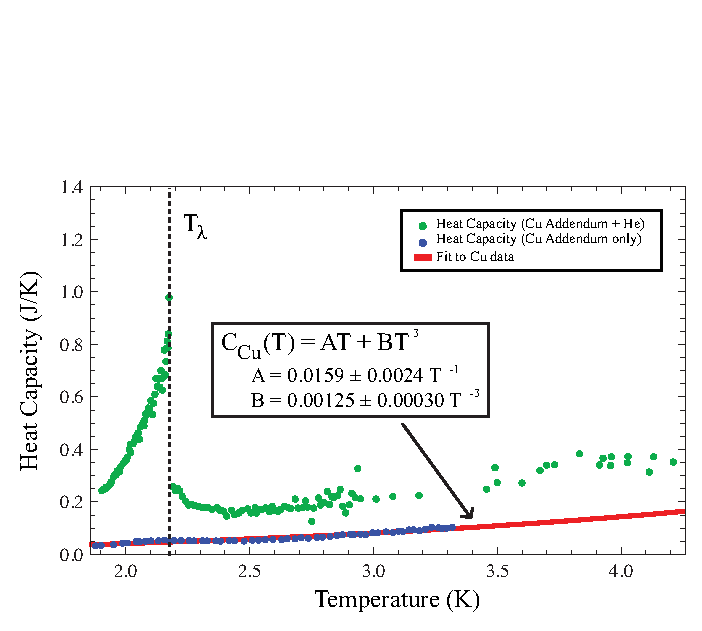
\includegraphics[height=80mm]{./figures/lambdanorm.eps}
\caption{\small{The heat capacity of the copper cell filled with He II and the heat capacity of the evacuated copper cell.  A polynomial with cubic and linear terms was fit to the copper data in order to ultimately remove the cell's contribution to the heat capacity data.}}
\label{fig:lambdanorm}
\end{center}
\end{figure}

To determine heat capacity of He without the copper cell we need to uniformly subtract heat capacity of the copper cell from the filled cell measurement.  To do this we fit a curve to the empty copper cell data.  At low temperatures, the heat capacity of copper is described by a combination of a linear and cubic term (see Section \ref{specificheatofmetals}).  Therefore we fit the copper heat capacity data to a $3^{rd}$-degree polynomial without  quadratic or constant terms using nonlinear regression.  We find that the heat capacity of the copper cell is given by

\begin{center}
\begin{equation}\label{eq:cufit}
C^{Cu}_{v} = 0.0159\pm0.0024 T+ 0.00125\pm0.00030 T^{3} 
\end{equation}
\end{center}

To remove the copper's contribution from the combined heat capacity at a specific temperature, we simply subtract the heat capacity of the cell, given by Equation \ref{eq:cufit}, for that temperature. Thus we are able to calculate the heat capacity of the He which is contained in the cell for the temperature region observed.  This heat capacity data must then be normalized to account for the amount of He in the cell. As described in Section \ref{heatcapacityexperiment}, by measuring the pressure of a certain volume of He at room temperature, we can use the ideal gas law to compute the number of moles of He in that volume.  That volume is then inserted into the cell through a capillary tubing.  We assume that almost all of the He is condensed in the cell due to the density of liquid helium being much greater than that of gaseous helium.  Knowing the number of moles of He in the cell, we can calculate its specific heat in J/mol K. This final data is shown in Figure \ref{fig:lambdatrans}.

\begin{figure}[htbp]
\begin{center}
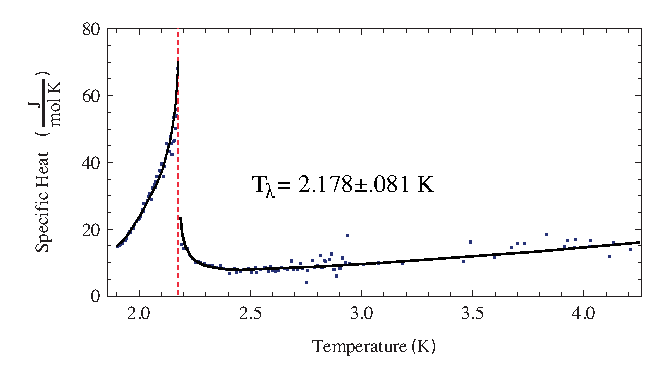
\includegraphics[height=80mm]{./figures/lambdatrans.eps}
\caption{\small{The specific heat of He II \emph{vs.} temperature. The transition from He I to He II occurs at $T_{\lambda} = 2.178 \pm 0.081$ K.  The values for specific heat each have a relative statistical error ranging from $10\%$  to $17\%$ based on the temperature of the helium (see Appendix \ref{errorinspecificheatcalculation} for error analysis). Our points are overlaid onto the result from Atkins \cite{atkins}.}}
\label{fig:lambdatrans}
\end{center}
\end{figure}

\subsection{Superfluid and Normal Fluid Densities}\label{superfluiddensity}


We use the second sound speed and specific heat measurements derived
in Sections \ref{secondsoundanalysis} and \ref{heatcapacityanalysis}
to derive the fractions of superfluid and normal fluid as a function
of temperature. Given the speed of second sound, the specific heat,
and the entropy of helium II, it is possible to derive the ratio of
superfluid to normal fluid densities, $\rho_s/\rho_n$ by using the
relationship in Equation \ref{soundspeed}. From this ratio it is
straightforward to find the fractions $\rho_s/\rho$ and $\rho_n/\rho$
where $\rho$ is total density, since from \ref{eqn:density} we have
$\frac{\rho_n}{\rho} = 1 - \frac{\rho_s}{\rho}$.

As our experiment did not measure the entropy of helium II, we use the
results of Brooks and Donnelly \cite{brooks}. The entropy
values are cited at pressures of $0.0$ atm, $2.50$ atm, and so on. Our
measurements were done at vapor pressures between $0.01$ atm and
$0.05$ atm, so the values for $0.0$ atm were used for the calculation.
In order to interpolate the entropy data, the logarithm of the
entropy, $\ln S$, was fitted to a second order polynomial:
\begin{equation}
\ln S = -0.8529T^2 + 6.092T - 8.82
\end{equation}

with an $r^2$-value of $0.9999$, which justifies the use of this fit
to interpolate entropy data.

In order to increase the precision of the specific heat data, between
$5$ and $10$ data points were averaged to give a value at each
temperature. The specific heat per gram 
and  the second sound velocity were combined with the entropy data to
find the fraction of superfluid and normal fluid
(Figure \ref{fig:density}). The curve can be seen to be in good agreement with
previously established results: most significantly the shape, position
of the $\lambda$-point, and the appromixate temperature where $\rho_s
= \rho_n$ are in correspondence with previous literature \cite{andro}.

\begin{figure}[htbp]
\begin{center}
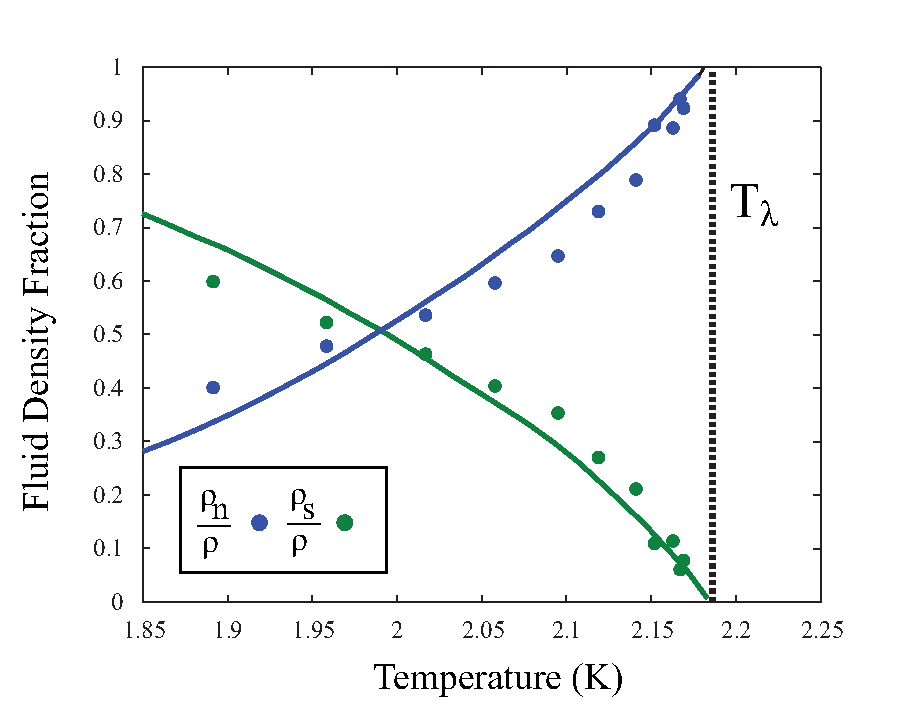
\includegraphics[height=70mm]{./figures/density.eps}
\caption{\small{Fraction of superfluid and normal fluid densities in
    helium II as a function of temperature, compared to
    Andronikoshvili's classic result from 1946 (solid
    line)\cite{andro}.}}
\label{fig:density}
\end{center}
\end{figure}


%Conclusion body
%Created MB 04-12

\section{Conclusion}\label{conclusion}

In this experiment, we observe several properties of liquid $^4$He and
compute important temperature-dependent functions of this unique
system. The fountain effect as well as the cessation of
bubbling at the $\lambda$-point are observed. Measurements of second sound
velocity and specific heat are in very good agreement with previous
results; the temperature of the $\lambda$-point was found to be
$T_{\lambda} = 2.178 \pm 0.081$ K which corresponds to the
experimentally established value of $2.17$ K. In addition, the
superfluid and normal fluid density fractions are derived from our
data and compare well to previously established values, demonstrating strong evidence for the accuracy of Landau's two-fluid model. Future
improvements to the system would include an improved pumping system
and further limiting thermal conductivity to the environment, which
would enable more precise results over a greater range of
temperatures, including the region where the fraction of superfluid helium approaches unity.





\appendix

\begin{center}
\begin{Large}
\bfseries{Appendices}
\end{Large}
\end{center}


%\addcontentsline{toc}{section}{References}
\newpage
\bibliography{writeup}
\bibliographystyle{abbrv}

\end{document}


